\chapter{System Design and Implementation} \label{ch:problem-solution}

This chapter describes the design and implementation of Pista, a GenAI-powered startup pitch evaluation system. The development addressed fundamental limitations in existing evaluation methodologies while establishing a research platform for systematic comparison with commercial evaluation methods. The implementation illustrates practical integration of GenAI into entrepreneurial assessment workflows.

\section{Solution Approach and Design Philosophy} \label{sec:solution-approach}

The Pista system was designed to address limitations in contemporary startup evaluation methodologies through standardized assessment frameworks enhanced with GenAI capabilities. The solution provides consistent, scalable evaluation while preserving the analytical depth required for entrepreneurial assessment.

Three fundamental limitations in existing evaluation methodologies were addressed:

\begin{itemize}
  \item \textbf{Scalability Constraints}: Automated processing eliminates cognitive fatigue effects that compromise human evaluator performance during extended assessment periods \cite{Hirshleifer2019}
  \item \textbf{Geographic Access Barriers}: Cloud-based platform provides access to evaluation capabilities regardless of geographic location, addressing expert evaluator concentration in major entrepreneurial centers \cite{Colombo2019}
  \item \textbf{Assessment Consistency}: Standardized evaluation framework applies uniform criteria across evaluations, reducing subjective variability found in traditional expert panel approaches \cite{Gius2024}
\end{itemize}

Multi-format input capabilities (text, audio, document uploads) accommodate diverse communication preferences while maintaining evaluation quality.


\section{System Architecture and Technical Implementation} \label{sec:system-design}

\subsection{Overall Architecture Design}\label{subsec:architecture-overview}
Pista was implemented as a three-tier web application. The presentation layer uses Next.js 15\footnote{\url{https://nextjs.org}} with React for responsive user interfaces. The application layer manages business logic through API routes, authentication services, and GenAI evaluation pipelines. PostgreSQL with Prisma ORM\footnote{\url{https://prisma.io}} provides type-safe database operations in the data layer.

The architecture supports both user experience and research requirements. Individual user workspaces provide data isolation while maintaining simple navigation. The design enables systematic comparison with commercial platforms through standardized criteria, multi-format inputs, and structured outputs suitable for quantitative analysis.

Several key services were integrated:
\begin{itemize}
  \item \textbf{NextAuth.js v5}\footnote{\url{https://next-auth.js.org}} providing secure authentication with OAuth provider support (Google, GitHub)
  \item \textbf{PostgreSQL with Prisma ORM} ensuring robust relational data management with ACID compliance and type safety
  \item \textbf{OpenAI APIs}\footnote{\url{https://platform.openai.com}} powering primary GenAI evaluation and audio transcription capabilities
  \item \textbf{Multi-Provider GenAI Integration} incorporating OpenAI GPT-4, Anthropic Claude, and Google Gemini for ensemble evaluation approaches
\end{itemize}

The technology selection criteria emphasized both performance and research requirements. Next.js 15 provides exceptional developer experience through built-in optimizations and React Server Components, enabling rapid iteration during development. PostgreSQL ensures evaluation data integrity through ACID compliance, critical for research reproducibility. NextAuth.js streamlines OAuth integration while maintaining enterprise-grade security standards. The multi-provider GenAI architecture reduces single-point-of-failure risks while enabling sophisticated ensemble evaluation techniques that improve assessment reliability \cite{Steyvers2024}.

The overall system workflow encompasses user interaction, data processing, and output generation as illustrated in Figure~\ref{fig:user-flow}.

\begin{figure}[H]
  \centering
  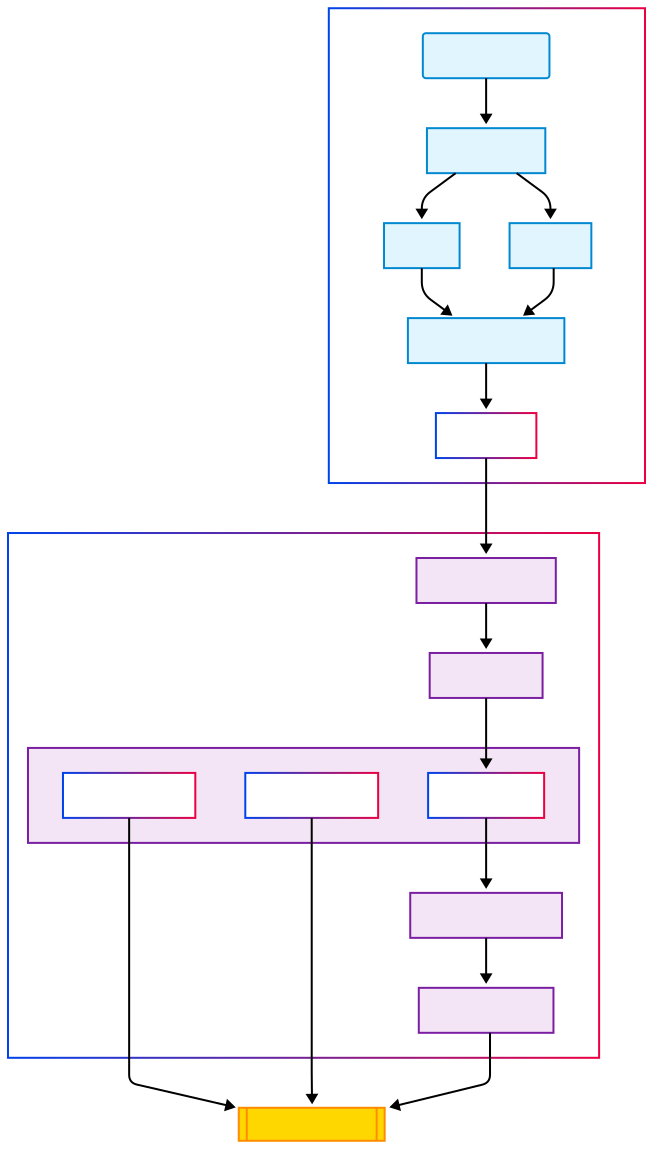
\includegraphics[width=0.85\textwidth]{img/user-diagram-flow}
  \caption{High-level system workflow showing user interaction and data processing stages}
  \label{fig:user-flow}
\end{figure}

\subsection{GenAI Evaluation Framework Implementation}\label{subsec:evaluation-framework}
The evaluation framework constitutes the core innovation of the system, developed through analysis of venture capital methodologies and evaluation literature. The implementation combines standardized criteria with GenAI prompt engineering to deliver consistent results.

\subsubsection{Framework Implementation}
A four-dimensional assessment structure was implemented through TypeScript configuration objects:

\begin{lstlisting}[language=TypeScript, caption=Core Evaluation Framework Configuration, label=lst:eval-framework]
const EVALUATION_CRITERIA = {
  problemSolutionFit: {
    name: "Problem-Solution Fit",
    aspects: [
      "Problem Definition Clarity",
      "Problem Significance and Market Pain",
      "Solution Feasibility and Innovation",
      "Product-Market Fit Evidence",
      "Customer Validation and Feedback"
    ]
  },
  businessModelMarket: {
    name: "Business Model & Market",
    aspects: [
      "Market Size and Growth Potential",
      "Revenue Model and Unit Economics",
      "Go-To-Market Strategy",
      "Competitive Landscape and Positioning",
      "Scalability and Market Timing"
    ]
  },
  teamExecution: {
    name: "Team & Execution",
    aspects: [
      "Founder and Team Capabilities",
      "Domain Expertise and Track Record",
      "Execution Ability and Progress",
      "Leadership Quality and Vision",
      "Resource Management and Adaptability"
    ]
  },
  pitchQuality: {
    name: "Pitch Quality",
    aspects: [
      "Communication Clarity and Structure",
      "Storytelling and Engagement",
      "Data and Evidence Presentation",
      "Funding Ask and Use of Funds",
      "Overall Persuasiveness"
    ]
  }
};

const WEIGHTS: Record<string, number> = {
  "Problem-Solution Fit": 0.30,
  "Business Model & Market": 0.30,
  "Team & Execution": 0.25,
  "Pitch Quality": 0.15
};
\end{lstlisting}

This structure captures objective and subjective assessment aspects. Equal weighting (30\% each) was applied to Problem-Solution Fit and Business Model as fundamental viability indicators. Team \& Execution receives 25\% weight reflecting execution importance, while Pitch Quality (15\%) emphasizes communication effectiveness \cite{Gompers2020}.

\subsubsection{Advanced Prompt Engineering Implementation}
The system's effectiveness depends critically on sophisticated prompt engineering that guides GenAI models toward consistent, high-quality evaluations. The prompt construction incorporates established venture capital evaluation practices and adapts to industry-specific requirements:

\begin{lstlisting}[language=TypeScript, caption=GenAI Prompt Engineering System, label=lst:prompt-engineering]
function buildPrompt(criteriaName: string, aspects: string[], 
                    fullContent: string): string {
  return `
As an expert startup evaluator, analyze this pitch focusing on ${criteriaName}.

Consider these specific aspects:
${aspects.map((aspect) => `- ${aspect}`).join('\n')}

Content to evaluate:
${fullContent}

Provide:
1. Score (1-10) with specific justification
2. Key strengths (3-5 bullet points)
3. Areas for improvement (3-5 bullet points) 
4. Detailed analysis of each aspect
5. Critical insights and recommendations
6. Actionable recommendations for the founder

Format your response as follows:
SCORE: [number]
STRENGTHS:
- [point 1]
- [point 2]
...
IMPROVEMENTS:
- [point 1]
- [point 2]
...
ANALYSIS:
[Your detailed analysis]
`;
}
\end{lstlisting}

The prompt engineering approach emphasizes structured output through system messages positioning the GenAI as an experienced evaluator. This methodology maintains consistent quality while preserving flexibility for diverse assessment scenarios.

\subsubsection{Industry-Specific Enhancement System}
The enhanced evaluation framework implements dynamic weighting adjustments based on automatically detected industry context and startup development stage:

\begin{lstlisting}[language=TypeScript, caption=Industry-Specific Weight Configuration, label=lst:industry-weights]
const INDUSTRY_PROFILES: Record<string, IndustryProfile> = {
  saas: {
    name: 'SaaS & Software',
    weights: {
      'Problem-Solution Fit': 0.25,
      'Business Model & Market': 0.35, // Emphasis on recurring revenue
      'Team & Execution': 0.25,
      'Pitch Quality': 0.15
    },
    specificCriteria: [
      'Customer acquisition cost (CAC)',
      'Monthly recurring revenue (MRR) growth',
      'Churn rate and retention',
      'Product-market fit indicators'
    ]
  },
  fintech: {
    name: 'FinTech',
    weights: {
      'Problem-Solution Fit': 0.30,
      'Business Model & Market': 0.30,
      'Team & Execution': 0.30, // Regulatory compliance emphasis
      'Pitch Quality': 0.10
    },
    specificCriteria: [
      'Regulatory compliance strategy',
      'Security and risk management',
      'Financial partnerships'
    ]
  }
};
\end{lstlisting}

This approach enables industry-specific evaluation reflecting venture capital practices while maintaining comparison capabilities with commercial platforms.

The evaluation processing workflow implements the four-dimensional assessment structure as shown in Figure~\ref{fig:eval-flow}.

\begin{figure}[H]
  \centering
  \includegraphics[width=0.9\textwidth]{img/eval-flow.png}
  \caption{Evaluation processing workflow showing four-dimensional assessment structure}
  \label{fig:eval-flow}
\end{figure}

\subsection{GenAI Integration Strategy}\label{subsec:ai-integration-strategy}
The evaluation engine integrates multiple GenAI providers (OpenAI GPT-4, Anthropic Claude, Google Gemini) through a unified interface. Multi-provider ensemble evaluation was designed to improve reliability and reduce individual model bias.

\subsubsection{Design Considerations and Limitations}
The system design acknowledges several important considerations that inform deployment strategies:

\begin{itemize}
  \item \textbf{Potential for Systematic Biases}: GenAI evaluation may exhibit consistent patterns in scoring that differ from human evaluator assessment approaches
  \item \textbf{Discrimination Capabilities}: Automated systems may show tendency toward score convergence rather than granular quality differentiation
  \item \textbf{Human Factor Assessment}: Limited ability to evaluate intangible aspects such as team dynamics, leadership presence, and execution track records
  \item \textbf{Risk Assessment Variations}: Possible differences in risk evaluation compared to experienced commercial evaluators
\end{itemize}

These considerations inform the system's role as a complementary tool rather than a replacement for traditional evaluation methods, supporting the research goal of understanding optimal deployment strategies for GenAI evaluation systems.

\subsubsection{Enhanced Evaluation Pipeline}
The enhanced evaluation system implements context-aware prompting that adapts to industry type, startup stage, and pitch format. The system automatically detects industry context from pitch content and applies appropriate evaluation weights and benchmarks.

The content processing pipeline architecture is illustrated in Figure~\ref{fig:eval-flow-context}.

\begin{figure}[H]
  \centering
  \includegraphics[width=0.85\textwidth]{img/eval-flow-context}
  \caption{Content processing pipeline with automatic context detection and industry-specific weight application}
  \label{fig:eval-flow-context}
\end{figure}

The content processing pipeline, illustrated in Figure~\ref{fig:eval-flow-context}, was designed to handle multiple input formats while automatically detecting industry context and startup development stage. Industry-specific weight profiles were established for major sectors, with each profile containing customized evaluation weights and benchmark scores derived from market research.

The enhanced evaluation system implements context-aware prompting that automatically detects industry type and startup stage, applying appropriate evaluation weights and benchmarks. The processing architecture supports both single-provider and ensemble evaluation modes through parallel dimension assessment.

\subsubsection{Multi-Provider GenAI Evaluation Architecture}
The GenAI evaluation processing was designed to support both single-provider and ensemble evaluation modes. The system architecture enables parallel processing across multiple GenAI providers while maintaining consistent evaluation criteria and output formats.

The GenAI evaluation processing architecture is detailed in Figure~\ref{fig:eval-flow-ai}.

\begin{figure}[H]
  \centering
  \includegraphics[width=0.85\textwidth]{img/eval-flow-ai}
  \caption{GenAI evaluation processing architecture showing parallel dimension assessment across multiple providers}
  \label{fig:eval-flow-ai}
\end{figure}

The evaluation processing architecture, depicted in Figure~\ref{fig:eval-flow-ai}, was implemented to process each dimension in parallel through either single-provider (GPT-4) or ensemble modes. The ensemble approach was designed to incorporate multiple GenAI providers (GPT-4, Claude, Gemini) with specialized personas to reduce individual model bias and improve assessment reliability.

\subsubsection{Industry-Specific Prompt Engineering}
The prompt engineering approach was enhanced to incorporate industry-specific criteria and stage-appropriate expectations. The system generates contextual prompts that position GenAI evaluators as domain experts familiar with specific industry standards and investment criteria.

Industry-specific weight profiles adjust evaluation emphasis based on sector characteristics. For example, SaaS platforms emphasize business model viability (35/%) due to subscription revenue models, while FinTech ventures require stronger team assessment (30%) due to regulatory environments.

\subsection{Data Models and Storage Architecture}\label{subsec:data-models-and-storage-architecture}
The data layer implements a comprehensive schema supporting users, pitches, and evaluations using PostgreSQL for relational data management with Prisma ORM for type-safe database operations. The schema ensures proper data isolation and security through user-scoped access controls.

\subsubsection{Database Schema Design}
The database schema includes core entities for users, pitches, evaluations, and user favorites. The schema implements proper foreign key relationships and cascading deletion policies to maintain data integrity.

The database schema implements core entities for users, pitches, evaluations, and user favorites with proper foreign key relationships and cascading deletion policies to maintain data integrity.

\subsubsection{User Architecture}
The system implements a streamlined user model focused on pitch management and evaluation. Each user's data is properly isolated within their account, providing a clean and focused experience. This approach prioritizes ease of use and immediate value delivery for entrepreneurs and startup founders.

\subsubsection{Research Methodology Support}
The system architecture directly supports the research methodology for systematic comparison with commercial evaluation platforms:

\begin{itemize}
  \item \textbf{Consistent Evaluation Framework}: The 4-dimension evaluation structure enables direct comparison with commercial platforms using different assessment criteria
  \item \textbf{Structured Data Collection}: All evaluations are stored with standardized scoring and feedback formats that facilitate statistical analysis
  \item \textbf{Multi-Format Input Support}: Text, audio, and file upload capabilities ensure comprehensive coverage of pitch submission methods
  \item \textbf{Reproducible Results}: Standardized prompting and evaluation processes enable consistent assessment across multiple pitches
\end{itemize}

This design enables empirical evaluation of GenAI system performance characteristics, bias identification, and deployment strategy development through systematic comparison with established commercial evaluation methods. The architecture supports controlled experiments with identical pitch content evaluated by both GenAI and commercial systems to identify systematic differences and optimal deployment strategies.


\section{Authentication and Authorization Implementation}

\subsection{NextAuth.js Integration Architecture}
The authentication system was implemented using NextAuth.js v5, supporting OAuth providers including Google and GitHub. The system employs JWT-based session management for scalability and implements user-based access control.

The authentication system uses NextAuth.js v5 with OAuth providers including Google and GitHub, implementing JWT-based session management for scalability and user-based access control.

\subsection{Access Control}
The system implements user-scoped data access through authentication middleware and API route protection. Each authenticated user has access to their own pitches, evaluations, and analytics. This permission model ensures privacy and security while maintaining ease of use.


\section{GenAI Processing Pipeline Implementation}

\subsection{Multi-Provider GenAI Integration Architecture}
The evaluation system integrates multiple GenAI providers including OpenAI GPT-4, Anthropic Claude, and Google Gemini through a unified interface. This multi-provider approach enables ensemble evaluation where multiple GenAI models contribute to the final assessment, improving reliability and reducing bias.

\subsubsection{Content Processing Pipeline}
The system supports multiple input formats including text, audio files, and document uploads. Audio processing utilizes transcription services, while document processing extracts and analyzes textual content through a standardized pipeline.

The content processing pipeline supports multiple input formats including text, audio files, and document uploads, with audio processing utilizing transcription services and document processing extracting textual content through a standardized pipeline.

\subsubsection{Enhanced Scoring and Benchmarking System}
The enhanced scoring system was implemented to apply dynamic weight adjustments based on detected industry context and startup development stage. The scoring pipeline incorporates benchmark comparisons and percentile calculations to provide contextual assessment relative to industry standards.

The enhanced scoring methodology is demonstrated in Figure~\ref{fig:eval-flow-scoring}.

\begin{figure}[H]
  \centering
  \includegraphics[width=0.85\textwidth]{img/eval-flow-scoring}
  \caption{Enhanced scoring methodology with industry-specific weight application and benchmark comparison}
  \label{fig:eval-flow-scoring}
\end{figure}

The scoring methodology, illustrated in Figure~\ref{fig:eval-flow-scoring}, was designed to calculate weighted scores using industry-specific profiles while generating comprehensive feedback including strengths identification, improvement recommendations, and industry-specific insights. This approach enables contextual evaluation that adapts to different industry requirements and startup development stages.

\subsubsection{Enhanced Evaluation Processing}
The enhanced evaluation pipeline implements context-aware processing with automatic industry detection and stage classification. The system includes comprehensive error handling with exponential backoff for API rate limiting and fallback mechanisms for service interruptions.

\section{User Interface and Experience Design}

\subsection{Component Architecture and User Experience Design}
The user interface was designed following modern UX principles with emphasis on accessibility, responsiveness, and progressive enhancement. The interface supports startup workflows with a focus on user-centric design.

\subsubsection{Core User Features}
The system provides several key features for managing and evaluating pitches:

\begin{itemize}
  \item \textbf{Dashboard with Multiple Views}: Users can view all pitches, recent submissions, favorites, and compare pitches side-by-side
  \item \textbf{Multi-Format Pitch Creation}: Support for text input, file uploads, and audio recordings with automatic transcription
  \item \textbf{Favorites System}: Users can mark pitches as favorites for quick access and comparison
  \item \textbf{Search and Filtering}: Real-time search across pitch content with filtering by score ranges and submission dates
  \item \textbf{Detailed Evaluation Results}: Comprehensive feedback with dimension-specific scores and improvement recommendations
\end{itemize}

\subsubsection{User Experience Implementation}
The system implements automatic workspace setup for new users upon authentication. The interface is designed to provide immediate access to pitch creation and evaluation features with a clean, intuitive navigation structure.


\subsection{Performance Optimization and Monitoring}
The system implements comprehensive performance monitoring and optimization strategies to ensure scalable operation under varying load conditions through custom performance tracking hooks and virtualized components for large datasets.


\subsubsection{Performance Tracking Implementation}
Performance tracking was implemented using custom hooks that monitor user interactions, component render times, and API response times. The tracking system provides insights into user behavior and system performance bottlenecks.

The system implements performance monitoring through custom tracking hooks that monitor user interactions, component render times, and API response times, providing insights into system performance and user behavior patterns.

\subsubsection{Virtualization for Large Datasets}
For large datasets, the system implements virtualization techniques to maintain responsive user interfaces through React virtualization for rendering large lists of pitches efficiently.



\section{Deployment and Infrastructure}

\subsection{Development and Production Environments}
The application supports multiple deployment environments with configuration management through environment variables. The development environment utilizes Next.js development server with hot reloading for rapid development cycles. Production deployment requires environment-specific configurations for database connections, GenAI provider API keys, and authentication secrets.


\subsection{Security Considerations}
The system implements several security measures appropriate for user data protection:
\begin{itemize}
  \item \textbf{Authentication}: Secure OAuth implementation through NextAuth.js with HTTPS-only cookies
  \item \textbf{Data Isolation}: User-scoped database queries prevent cross-user data access
  \item \textbf{Input Validation}: Server-side validation and sanitization of all user inputs
  \item \textbf{API Security}: Rate limiting and request validation for GenAI provider endpoints
\end{itemize}






\section{Implementation Results and System Validation}
\label{sec:results}

The implemented system demonstrated consistent performance characteristics suitable for research evaluation and practical deployment. This section presents key implementation outcomes and validation results that inform the comparative evaluation presented in Chapter 4.

\subsection{System Performance Characteristics}
\label{subsec:performance}

Text-based pitch evaluations were completed within 30-60 seconds, while audio submissions required additional processing time for transcription. The multi-provider architecture supported concurrent evaluations, enabling systematic comparison studies. Database operations maintained sub-100ms response times for typical user interactions, ensuring responsive user experience during evaluation workflows.

\subsection{Multi-Format Input Validation}
\label{subsec:input-validation}

The pitch submission workflow successfully accommodated diverse input formats through direct text entry, file uploads (PDF, DOCX), and audio recordings. Transcription accuracy exceeded 95\% for clear audio recordings, though performance degraded with background noise or multiple speakers. The enhanced evaluation system with industry-specific weights provided contextually appropriate assessments compared to generic evaluation approaches.

\subsection{Research Architecture Validation}
\label{subsec:research-validation}

The modular architecture enabled systematic evaluation research through independent components for authentication, evaluation, and data management. Standardized data collection facilitated statistical analysis of evaluation patterns. The separation between standard and enhanced evaluation approaches supported comparative analysis across different GenAI configurations, providing the foundation for the empirical evaluation presented in the following chapter.
